\newsection
\subsection{Environment}
\label{sec:environment}
\sectionauthors{Peter Henderson, Lauren Gillespie, Dan Jurafsky}

\begin{figure}[!ht]
\centering
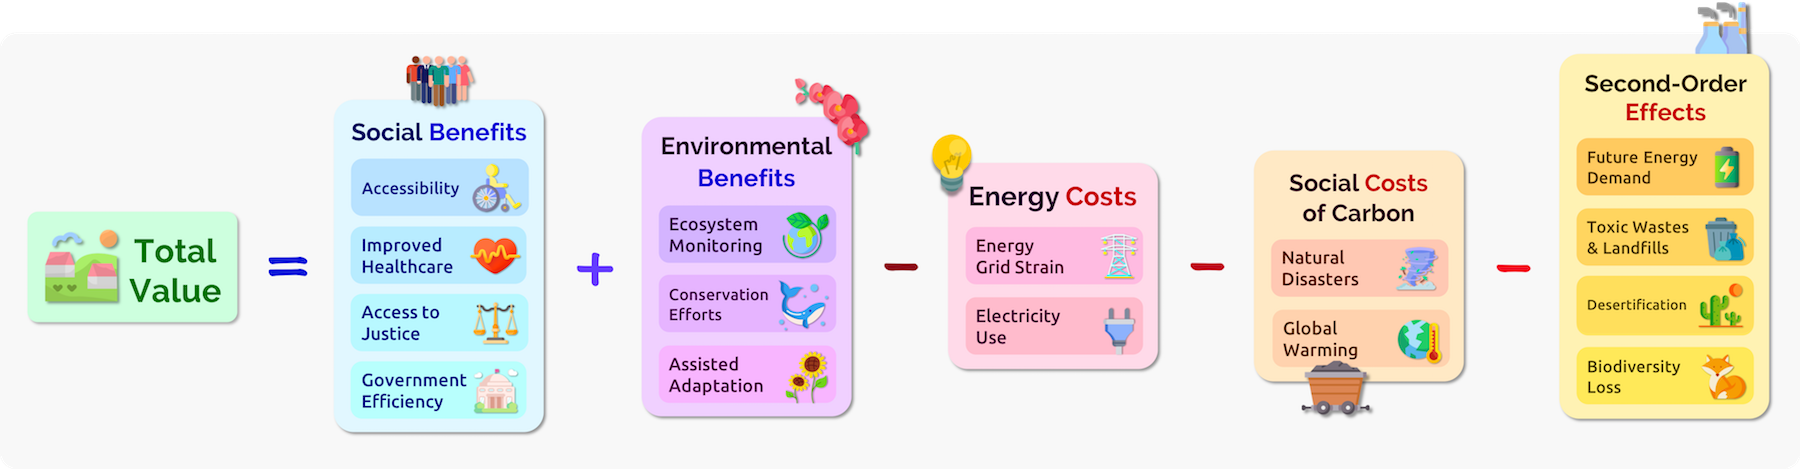
\includegraphics[width=\linewidth]{society/figures/Environment_Equation.png}
\caption{\label{fig:environment} A visualization of a cost-benefit analysis for deploying a foundation model. The total value of a model can be approximated by first considering the net positive social benefits of the model, as well as any environmental benefits. Then, we subtract the negative energy costs to train and deploy the model, the social cost of the carbon emitted to train the model, and the secondary environmental effects. If the net costs outweigh the benefits, then foundation model developers and large-scale deployers should consider harm reduction strategies. This could include deploying a more efficient model or not deploying the model at all. }
\end{figure}

Foundation models can potentially lead to many social and environmental benefits, for example in legal domains (\refsec{law}), healthcare (\refsec{healthcare}), or even tackling climate change~\citep{rolnick2019tackling}. But because of their scale, they themselves can negatively impact the environment through increased carbon emissions if model creators are not careful~\citep{strubell2019energy,lottick2019nergy,schwartz2019green,lacoste2019quantifying,cao2020towards,henderson2020towards,bender2021,patterson2021carbon,lannelongue2021green,parcollet2021energy}. Addressing such emissions is an imperative: current forecasts show that climate change is occurring more rapidly than previously thought~\citep{ipcc2021}.

To understand where such emissions can occur in foundation models, we consider their lifecycle. First, they are trained on vast amounts of data, possibly for up to months of time and often distributed across hundreds to thousands of GPUs. Afterwards, they may be adapted to new domains or perhaps distilled into smaller models. All of this can be considered part of the training regime. Models used purely for research may not move beyond these steps. 
After models have been adapted and/or distilled, they might move on to be deployed into production. At this point many rounds of inference will run through the model until a new model is trained and the cycle repeats. 

Each one of these steps has the potential to utilize large amounts of energy and can contribute to carbon emissions. Foundation models can generate large, one-time energy costs and carbon emissions during the initial training phase. For example, the amount of emissions from training one BERT-base model, under some conditions, would only be offset by 40 trees grown for 10 years.\footnote{\citet{strubell2019energy} calculate carbon emissions for training BERT on an average energy grid in the U.S. and we use \url{https://www.epa.gov/energy/greenhouse-gas-equivalencies-calculator} to convert that to equivalent emissions in other domains. We note that this number can vary depending on the energy grid and other considerations~\citep{henderson2020towards,patterson2021carbon}.}
And if deployed at scale, foundation models can require substantial energy to service millions of requests\footnote{For example, transformers are already used at scale for search both at Microsoft and Google. See \url{https://www.blog.google/products/search/search-language-understanding-bert/} and  \url{https://azure.microsoft.com/en-us/blog/microsoft-makes-it-easier-to-build-popular-language-representation-model-bert-at-large-scale/}.}\dash{}translating to large carbon emissions if nonrenewable resources are used.

Therefore, the environmental impacts of certain design decisions for both training and deploying foundation models can be substantial. 
Even seemingly minuscule decisions, like reducing the number of layers a model has, may lead to significant environmental cost reductions at scale. 
For example, based on calculations from \citet{henderson2020towards}, a slightly more energy efficient translation model deployed at the scale of a commercial translation service could save between 78 kgCO2eq and 12,768 kgCO2eq of carbon emissions \textit{per day} depending on the energy grid used.
This is roughly equivalent to the carbon sequestered by 1 to 211 trees grown for 10 years, or the carbon sequestered by .35 to 57.4 acres of forest in one year.\footnote{Sequestration estimated via \url{https://www.epa.gov/energy/greenhouse-gas-equivalencies-calculator}, but may be larger depending on other estimation methods. More efficient energy grids will emit less carbon, resulting in wide estimated ranges of impacts.}
Thus the design, deployment, and post-deployment monitoring of foundation models should adequately reflect these risks.

There are of course uncertainties in calculating the amount of energy used or carbon emitted by any given model~\citep{henderson2020towards,cao2020towards,patterson2021carbon}, and other sources of emissions may currently be much greater than those generated by foundation models~\citep{mora2018bitcoin}. But if foundation models continue to scale and gain in popularity, they may very well become a significant contributor to carbon emissions. 
Our goal is to provide a framework for foundation model developers and large-scale deployers\footnote{We focus on model developers and large-scale deployers, like those who build production systems on top of foundation models, because they are most able to make meaningful changes to reduce energy use and carbon emissions. A single change by these actors\dash{}like using a more efficient model\dash{}can scale to massive carbon savings, which would otherwise require a massive campaign to reach all downstream model users.} to consider how they can mitigate any unnecessary carbon emissions and keep the net social impact of these models positive.
We recommend that: 
\begin{enumerate}
    \item Carbon impacts can and should be mitigated in many cases. This can be accomplished by training models in low-carbon intensity regions,
    or by using more efficient models and hardware (\refsec{environment-mitigation}).
    \item When all mechanisms for mitigation have been exhausted and mitigation is no longer possible, 
    the costs and benefits to society should be assessed 
    to determine if and when a larger foundation model should be deployed over a smaller, more efficient, model 
   \dash{}with the understanding that the up-front costs of a large foundation model may be amortized over the lifetime of the model (\refsec{environment-costs}).
    \item Energy, computational, and carbon costs\dash{}as well as any efforts taken to mitigate negative impacts\dash{}should be clearly reported to inform policymaking and research (\refsec{environment-reporting}).
\end{enumerate}

\subsubsection{Carbon impacts can and should be mitigated in many cases}
\label{sec:environment-mitigation}
The  carbon impacts of training foundation models differ from the impacts of deploying them for inference.
Model training has no latency requirements, so  training  can be moved across energy grids with relative ease in cloud environments. 
Every energy grid has its own carbon intensity\dash{}the amount of carbon emitted per kilowatt-hour of energy used. For example, Qu\'ebec has an extremely low carbon intensity due to its reliance on hydroelectricity, while Estonia's energy grid has an extremely high carbon intensity due to its reliance on shale oil (though that is changing quickly)~\citep{henderson2020towards}.
Recent research has even suggested that the top 5\% of polluting power plants contributed 73\% of all electricity-based emissions~\citep{grant2021reducing}.
Thus, while training foundation models can be quite energy intensive, researchers have demonstrated that the carbon impacts of these models can be partly mitigated by \textit{selecting energy grids with minimal carbon emissions}~\citep{henderson2020towards,lacoste2019quantifying,patterson2021carbon}. 

\textit{Carbon offsets} have also been proposed as a stopgap until carbon-free renewable electricity is available at all data centers. This strategy involves reducing carbon emissions in one activity to offset the emissions from another. But most\dash{}if not all\dash{}carbon offsets are a strictly worse solution than not emitting CO$_{2}$ in the first place \cite{holl_tree_2020}. Some carbon offset programs can even have a negative impact. For example,  studies of forest planting campaigns (often a source of carbon offsetting) show that they can do more harm than good. They can yield monocultures (the use of one particular species of tree) that diminish the biodiversity of the region and reduce carbon storage in the forest soil~\citep{heilmayr2020impacts,hong2020divergent}. This could result in more carbon emissions when using carbon offsets than if the original carbon had never been emitted in the first place.
Therefore, when training or deploying a foundation model, we recommend designing for as little carbon emission as possible up-front, rather than simply relying on carbon offsets to cancel emissions.

When it is not possible to run in low-carbon regions, other mitigation strategies should be leveraged, reducing unnecessary energy usage. This includes:
\begin{itemize}
    \item using more efficient hardware,\footnote{Notably, California now regulates computers with inefficient GPUs for this reason, requiring that they stay below 30-100 kWhs/year, depending on the manufacturing date and computer type. \emph{See} Sections 1601-1608 of California’s Appliance Efficiency 
Regulations (Title 20).}
\item using mixed-precision training~\citep{micikevicius2017mixed} or quantization~\citep{gholami2021survey},
\item using more efficient architectures (\eg using an evolved transformer over a vanilla transformer architecture; or using sparse models)~\citep{pmlr-v97-so19a,patterson2021carbon,mostafa_parameter_2019},
\item distilling models and using distilled models (\eg~\citep{sanh2019distilbert}),
\item and utilizing other optimization strategies that will reduce energy costs (see more discussion in \refsec{systems}).
\end{itemize}

Maintainers of open source projects and cloud compute should strive to set their default settings to the most efficient possible, since ``green defaults'' are known to be the most effective mitigation strategies (see discussion in ~\citep{henderson2020towards}).
Other mitigation strategies can be found in recent literature~\citep{strubell2019energy,lacoste2019quantifying,schwartz2019green,henderson2020towards}.
We also note that reducing and mitigating energy usage also has the added benefit of making models more accessible to those with limited compute access (see \refsec{ethics} for more discussion).

However, when a model is mainly used for inference, \eg  deployed in a production application, it often cannot be moved to a less carbon-intensive energy grid for low-latency applications. 
In addition to using the mitigation strategies specified above, in this case it is important to weigh
the benefits of the proposed foundation model versus a more energy efficient alternative. We discuss this further in the subsequent section.

\subsubsection{Costs and benefits should be assessed before using foundation models}
\label{sec:environment-costs}

After taking as many steps as possible towards mitigation (or where mitigation is not possible),
it is vital to assess the required size of a foundation model\dash{}or whether a foundation model should be used at all. This cost-benefit analysis should consider:

\begin{enumerate}
    \item Is the social cost and environmental cost from deploying the foundation model greater than the social benefit of the model?
    \item Would another, computationally simpler and cheaper approach achieve comparable social benefit (\eg a much more efficient foundation model, or perhaps simple baseline)?
\end{enumerate}

A simplified scheme for assessing this trade-off considers the overall impact of a model $M$ as:

\begin{equation}
\label{eqn:env}
    V(M) = S(M) - C(M) - E(M) - O(M).
\end{equation}

\reffig{environment} represents this equation and the costs and benefits that may enter each variable. Here, $M$ is the model and $S$ is the net social benefit, as well as environmental benefit, in dollars. $S$ can be increased by improving healthcare, access to justice, decreasing poverty, improving environmental monitoring, aiding ecosystem conservation efforts, and so on. 

$C$ is the social cost of carbon from energy use. This represents the future harm to society from the carbon released as a present-day monetary value. The upper bound U.S. Environmental Protection Agency (EPA) estimate from 2017 for the social cost of carbon was \$105 (in 2007 U.S. dollars) per metric ton of $\text{CO}_2$ emitted.\footnote{See \url{https://19january2017snapshot.epa.gov/climatechange/social-cost-carbon_.html}. But note that the social cost of carbon can be a contentious metric~\citep{stern2021social}. By using a favorable discount factor, one can reduce carbon costs. As such, it can the calculation of this metric can vary across methodologies.} 

$E$ is the energy cost of the model. For example, in April 2021, the average U.S. residential energy cost was about \$0.1376 per kWh.\footnote{\url{https://www.eia.gov/electricity/monthly/epm_table_grapher.php?t=epmt_5_6_a}} Added to this variable could be the costs from increased strain on the energy grid. For example, a recent study suggested that the cost per energy grid interruption event, normalized by average demand, could be as high as \$15.9 per average kW~\citep{sullivan_updated_2015}.\footnote{Like the social cost of carbon, calculation of these costs can fluctuate across modeling methodologies.}

$O$ is the social cost of other second order environmental effects. This could include:
\begin{itemize}
    \item The compounding carbon impacts from increased chip demand and chip production~\citep{gupta2021chasing}.
    \item Other environmental impacts of chip manufacturing, like the creation of toxic waste sites in 
 Silicon Valley, whose health effects are unequally distributed to socially vulnerable populations~\citep{stewart2014uneven}, or pollution from manufacturing in Taiwan that has been linked to chronic health problems~\citep{tu2009ineffective,lin2016increased}. 
 \item The compounding effects of climate change that are not already included in the SCC model. For example, these effects could include accelerated desertification~\cite{huang_accelerated_2016}, rapid ecosystem changes that put many species at risk of extinction~\cite{urban_accelerating_2015}, and increased carbon emissions due to melting permafrost~\citep{schuur_climate_2015}. 
 \item Unnecessary strain on chip production capacities. Recent chip shortages have led to work stoppages in automobile manufacturing.\footnote{\url{https://www.reuters.com/business/autos-transportation/ford-shut-some-n-american-plants-few-weeks-chip-shortage-2021-06-30/}} There is no evidence to suggest that increasing demand for ML-optimized chips led to this shortage.\footnote{Though recent reports have suggested that demand for datacenter chips have surpassed the gaming sector. \emph{See} \href{https://www.nextplatform.com/2020/08/21/the-local-maxima-ascension-of-datacenter-at-nvidia/}{https://www.nextplatform.com/2020/08/21/the-local-maxima-ascension-of-datacenter-at-nvidia/}.}
 But such considerations fall into second order effects, where researchers might weigh whether the risks, however slight, of contributing to such negative impacts are worth using or deploying a large model.\footnote{Like for other metrics described previously, there is uncertainty as to how these impacts might be calculated and attributed to models.}
\end{itemize}

It is important to consider in this analysis that the economic benefits and social costs of carbon could be distributed unequally across communities, with poorer communities being impacted more heavily by climate change and wealthier communities being benefited by a model~\citep{bender2021}.\footnote{See also, \url{https://www.un.org/sustainabledevelopment/blog/2016/10/report-inequalities-exacerbate-climate-impacts-on-poor/} and \url{https://blogs.imf.org/2020/12/02/how-artificial-intelligence-could-widen-the-gap-between-rich-and-poor-nations/}.} As such, when conducting the Equation~\ref{eqn:env}  analysis, one should consider the benefits and harms to society more broadly rather than for a given organization or country. In this case $V(M)$ can be viewed as a distribution and should ideally be evenly distributed across the population. In cases where the distribution is highly uneven\dash{}for example where all the benefits fall to the model designer while all the harms fall to populations that will never benefit from the model\dash{}the designer should spend substantially more effort on mitigation before deploying the model. 

There is, of course, some uncertainty in which methodology to use when valuing each component of Equation~\ref{eqn:env}. 
Empirical estimates for many of these terms can range in multiple magnitudes depending on the data source and modeling choice for the phenomena, such as the different mechanisms for evaluating the social cost of carbon. The key takeaway of this cost-benefit analysis, however, is not the dollar valuation of each term in the equation, but rather the \emph{existence of} and relative importance of each of these effects. 
Our goal is to provide a high-level framework for beginning to consider these trade-offs. 
Future research may give more guidance on how to quantify each of these values. 

\begin{figure}[t]
    \centering
    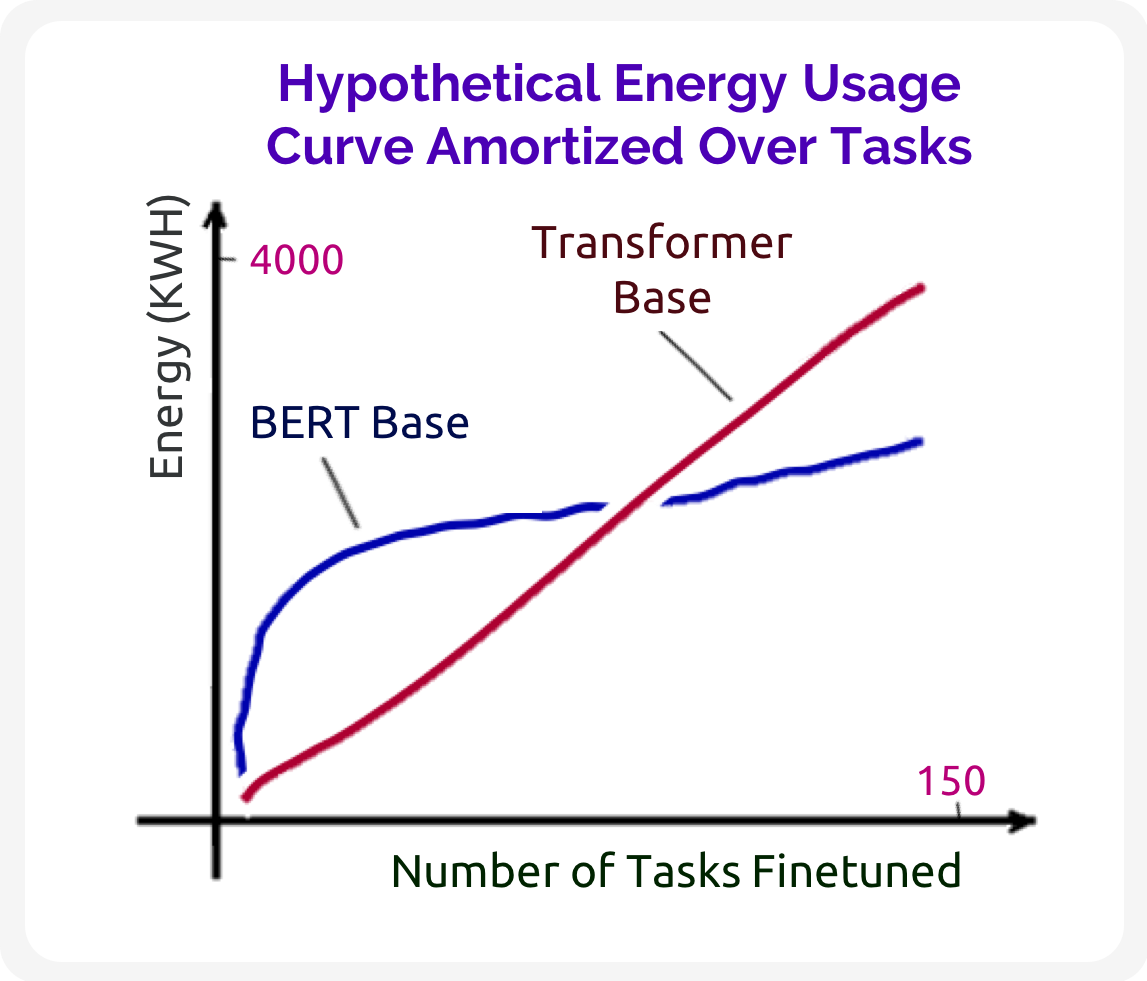
\includegraphics[width=.55\textwidth]{society/figures/Environment_Plot.png}
    \caption{A hypothetical example of amortized fine-tuning showing the point at which a foundation model (in this case BERT Base) will have lower energy costs than a transformer model trained from scratch. We estimate the up-front energy cost for training BERT from~\citet{strubell2019energy}, and cost for fine-tuning a downstream task from~\citet{chaudhary2020topicbert}. We compare against the linearly increasing cost of training a transformer from scratch, from~\citet{strubell2019energy}. If BERT is used for less than $\sim$80 tasks, the up-front energy costs are not recovered. After that point, BERT is  more energy efficient than the model trained from scratch.}
    \label{fig:env_bert_fine-tune}
\end{figure}

Finally, we note that these factors should also be evaluated over the lifetime of the model, not on a per-run basis. Consider an alternative baseline model that must be trained from scratch for every new task. The baseline may well require an expensive hyperparameter search to achieve equivalent performance on downstream tasks. In contrast, the foundation model places the brunt of the costs on the initial pretraining procedure, with fine-tuning perhaps being much simpler and more energy efficient. Over the lifetime of the foundation model, it could be more carbon efficient than the baseline  (\reffig{env_bert_fine-tune}). 
Even more efficient adaptation mechanisms could improve this amortization further (see \refsec{adaptation}).

The efficiency of adaptation, however, is not guaranteed. It may be true that some foundation models will never be more efficient than a particular baseline, even when amortized over many tasks.
For example, it cannot be assumed that a smaller model with fewer parameters will translate to energy efficiency improvements. Due to increased hyperparameter tuning costs or other optimizations, the number of parameters has been shown not to correlate with energy efficiency in some cases~\citep{zhou2020hulk,henderson2020towards}.
Therefore, foundation model developers should rigorously assess the efficiency of their models and adaptation mechanisms before beginning large-scale training efforts.

The framework in this section is meant to guide the reader in thinking about the environmental and societal trade-offs in training and deploying their model, but there are other substantial social justice considerations involved in deploying a foundation model, discussed in \refsec{ethics}.
\refsec{economics} also discusses in more detail the dynamics of social welfare from algorithm deployment.

\subsubsection{Carbon/energy impacts should be systematically reported}
\label{sec:environment-reporting}

A cost-benefit analysis cannot be conducted unless researchers and engineers working on foundation models report the computational, energy, and carbon costs of their models.
We encourage foundation model developers, providers, and curators to report these metrics, as well as what carbon reduction strategies were used in the making of the foundation model. 
See \citep{henderson2020towards,lottick2019nergy,lacoste2019quantifying,codecarbon,anthony2020carbontracker} for examples of a Carbon Impact Statement and for tools that can facilitate this reporting.
For researchers, such reporting can occur at publication time, but we also encourage industry actors to adopt transparency mechanisms to report these metrics for their deployed models.\footnote{A small step toward this has been taken by some cloud compute providers that identify the most carbon friendly cloud regions. See, for example, \href{https://cloud.google.com/blog/topics/sustainability/pick-the-google-cloud-region-with-the-lowest-co2}{https://cloud.google.com/blog/topics/sustainability/pick-the-google-cloud-region-with-the-lowest-co2}.}
This will help set policy recommendations within industry and academia, as well as help downstream users identify carbon-friendly usage patterns.
Standardized reporting will also aid in determining which models are accessible to those with limited compute access (see \refsec{ethics} for more discussion on accessibility).

To encourage more reporting of energy and carbon impacts, we suggest, among other strategies: giving green badges at conferences, requiring reporting of relevant metrics for submission to conference venues, lobbying large-scale deployers of foundation models to provide more transparency, and generally shifting professional norms in academia and industry towards standard reporting of these metrics (see more discussion on professional norms in \refsec{ethics} and more discussion on reporting mechanisms by \citet{henderson2020towards}).